\begin{problem}{神秘信号}{神秘信号.in}{神秘信号.out}{1 seconds}

难得在我的学习欲望达到最高点的绝佳时机,却被春日拉住袖子,硬是带到计算机中心301室去。

“你看看这个。”

春日边说边指给我看的,是之前从光电楼抢来的电脑屏幕。

我没办法反抗,只好乖乖地看了。绘图软件显示出一些我看不懂的涂鸦。在一个圆圈当中,有一些好像喝醉酒的绦虫蜷曲在一起形成的鬼东西,不知道是图是字还是什么象形文字,看起来就像幼稚园小朋友画出来的东西。

“这是我们SOS团的徽章。”

春日回答,露出完成了伟大成就似的得意表情。

“徽章?”我问道。

“没错,徽章。”春日说。

“这个吗?这种东西看起来就像熬夜一整晚、连续两个月连休假日也要刷题、一直AC不了的ACMer,一边喝小酒解宿醉一边走路留下来的脚印。”

“你看清楚啦!你瞧,正中央不是画了SOS团吗?”

经她这么一说,我仔细一瞧,这个东西不知道是不是心理作用、看起来也不能说不像SOS团、但是又不敢大声肯定是什么东西。以上我到底用了几个否定句呢?我自己是懒得算了,哪个吃饱没事干的人帮我算一下。

\begin{center}
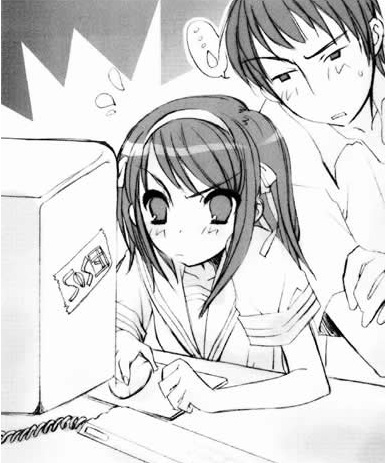
\includegraphics[width=0.4\textwidth]{pics/G.jpg}
\end{center}

“最闲的不就是你吗?反正考试时你也不念书的。”

刚刚我还充满想好好念书的冲劲。不过听她这么一说,事实倒也是这样。

“我想把这个登在SOS团网站的首页。”

经她这么一提,我想起确实是有这个东东。虽然是只有首页的可怜网站。

(附上网站地址 http://www.haruhi.tv/ 很遗憾比赛时身处局域网的您并不能看到这一伟大工程)

"你制作的这个网站,真是一点用处都没有,完全没有能够炒热气氛的东西。所以我就想到了,如果贴上SOS团的象征或者1096的照片之类的东西,会不会比较好一点?”

春日为了增加社团的热度,打算把 $n$ 张1096的照片放到网站上博人眼球。

但是我是绝对不允许的!况且,服务器还要一边判题,一边承受压力测试,哪有这么多资源给你自由发挥。

在我的强烈反对下,春日只能在满足不超过资源限制的情况下,最多挑 $n$ 张当中的 $m$ 张了。可恶,这根本就是不听取我的意见啊!

还是请你求出网站能获得的最大热度吧。

\InputFile

第一行三个正整数 $n,m,s (1 \leq n \leq 100 , 1 \leq m \leq min(50,n) , 1 \leq s \leq 500 )$ ,分别表示照片总数,最多可选的照片数与服务器可用资源数。

接下来 $n$ 行,每行包含两个正整数 $a_i,b_i (1 \leq a_i \leq 20 , 1 \leq b_i \leq 10^7)$ ,表示第 $i$ 张照片所要消耗的资源和会产生的热度。 

\OutputFile

一个整数表示网站能获得的最大热度。

\Example
\begin{example}
\exmp{
3 2 10
5 10
6 12
3 1
}{
13
}%
\end{example}
\end{problem}
